\documentclass{article}
\usepackage[utf8]{inputenc}
\usepackage[utf8]{inputenc}
\usepackage[spanish]{babel}
\usepackage{graphicx}
\title{}
\author{}
\date{}
\pdfinfo{%
  /Title    (Inteligencia Artificial I - Proyecto III)
  /Author   (Fabio Castro, María Jorge, Jorge Marcano)
  /Creator  ()
  /Producer ()
  /Subject  ()
  /Keywords ()
}
\begin{document}




 
\title{\Huge Inteligencia Artificial I\\ Proyecto III}



\author{Fabio Castro 10-10132, María Jorge 11-10495, Jorge Marcano 11-10566} 



\date{22/06/2015}

\maketitle

\section{Introducción}
\hspace{0.5cm}
El objetivo de este proyecto fue estudiar y utilizar el lenguaje de modelación de restricciones y \textit{"solver"} MiniZinc para solucionar varios problemas. Además de modelar los problemas, se utilizaron los \textit{"solvers"} provistos por MiniZinc para buscar las soluciones correspondientes a cada uno de ellos. A continuación se presentarán en detalle los resultados obtenidos en cada problema.


\section{Ejercicios}
\hspace{0.5cm}
\subsection{Ejercicio 1}

Este problema consistía en conseguir dígitos distintos mayores a cero para los símbolos {A,B,C,D,E,F,G,H,I} tal que la siguiente ecuación se cumpliera:
\begin{equation}
\frac{A}{B*C} + \frac{D}{E*F} + \frac{G}{H*I} = 1
\end{equation}

La implementación de este problema consistió en utilizar nueve variables de decisión (variables cuyos valores son asignados al momento de ejecutar el modelo, cumpliendo con las restricciones planteadas) para representar cada una de las nueve letras presentes en la ecuación. Se agregaron restricciones para asegurar que cada una de las letras tuviera un valor único respecto a las otras, y se cumpliera la ecuación.

Para este ejercicio se utilizó el \textit{solver} Gecode(bundled) provisto por MiniZinc y los resultados obtenidos, en un tiempo de 81msec, fueron los siguientes:\\
\begin{center} $A = 1$, $B = 6$, $C = 3$, $D = 5$, $E = 9$, $F = 8$, $G = 7$, $H = 4$ \end{center}

\subsection{Ejercicio 2}

El ejercicio 2 consistió en solucionar un juego colocando dígitos del 1 al 7 en cada posición vacía de forma tal que no existieran dígitos repetidos en alguna columna, fila o camino.

Para la implementación de este ejercicio decidimos representar el tablero como una matriz de tamaño 7x7 de números enteros entre el 1 y el 7. \par


Sobre este tablero, aplicamos las restricciones de que las columnas sean todas distintas entre si, y lo mismo
para las filas. Para hacer esto, utilizamos la función alldifferent, la cual, dado un arreglo y un rango de sus
elementos,se garantiza que los elementos dentro de ese rango serán distintos entre si. \par


Para aplicar las restricciones sobre los 7 caminos, creamos 7 arreglos de enteros entre 1 y 7 que representan los caminos, y
verificamos que cada miembro de cada camino sea igual a su posición en el tablero original, y colocamos otras restricciones
adicionales usando alldifferent para asegurarnos que los elementos de cada camino sean distintos entre si. \par


Al correr el programa con dichas restricciones, utilizando el \textit{solver} Gecode, obtuvimos el siguiente resultado en 19msec : 

\begin{figure}[!ht]
\begin{center}
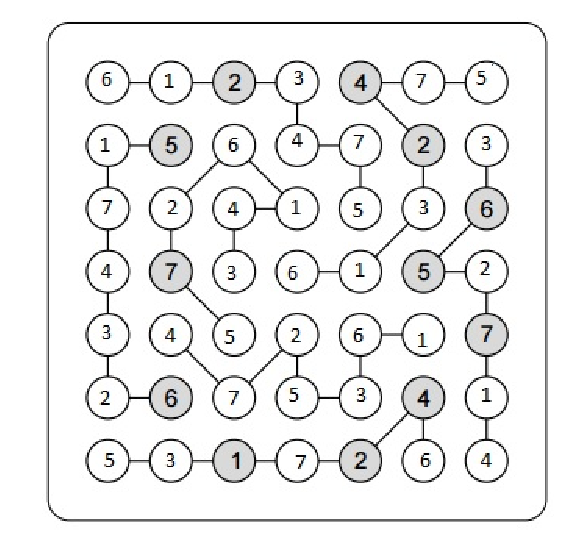
\includegraphics[width=0.9\textwidth]{salida2.eps}
\end{center}
\end{figure}

\subsection{Ejercicio 3}

Para este ejercicio debíamos encontrar la diferencia positiva más pequeña de dos números positivos de la forma $ABCDE - FGHIJ$ donde todos los dígitos \{0,1,...,9\} deben usarse, es decir, cada letra debe reemplazarse por un dígito distinto.

Al igual que en el Ejercicio 1 se usaron variables de decisión para representar cada letra en \{A,B,C,D,E,F,G,H,I,J\} (diez variables de decisión en total), cada una con un rango de posibles valores entre 0 y 9, debido a que representan dígitos. Se agregaron restricciones para asegurarnos de que cada letra tuviera asignado un dígito diferente (usando la función \textit{alldifferent}) y para verificar que la diferencia entre los dos números sea positiva. Finalmente, para garantizar que esta diferencia es la más pequeña existente, utilizamos \textit{solve minimize} para minimizar el resultado.

Los resultados obtenidos utilizando el \textit{solver} Gecode en 923msec fueron:
\begin{center}
$A = 5$, $B = 0$, $C = 1$, $D = 2$, $E = 3$, $F = 4$, $G = 9$, $H = 8$, $I = 7$, $J = 6$
\end{center}
Generando así los números 50123 y 49876, que al restarlos da como resultado 247.

\subsection{Ejercicio 4}

En este ejercicio se quería determinar el menor número de ascensores tales que las instalaciones sean eficientes (es posible ir entre dos pisos cualesquiera en un sólo viaje con al menos un ascensor). Para esto, utilizamos una matriz cuyas filas corresponden al mínimo de ascensores y las columnas los pisos del edificio. La posición [i,j] de la matriz tendrá un 1 si el ascensor i se para en el piso j, y 0 en caso contrario. Estas asignaciones son las que tiene que buscar el \textit{solver} al momento de ejecutar el modelo. 

El modelado consiste en cuatro restricciones: las primeras dos permiten fijar las paradas en el primer y en el último piso de cada ascensor, luego una restricción que para cualquier par de pisos del edificio, verifica que exista al menos un ascensor que pueda ir de uno a otro, y finalmente una restricción para asegurarnos que cada ascensor tenga exactamente k + 2 paradas (el primer piso, el último y los k pisos adicionales que deben asignarse).

Para determinar el número mínimo de ascensores necesarios se realizaron corridas fijando un m (empezando desde m = 1) y aumentándolo de uno en uno hasta que el problema pudiera resolverse.

Como en los ejercicios anteriores el \textit{solver} utilizado fue Gecode, y los resultados obtenidos para cada caso son los siguientes:

\begin{itemize}
\item Caso (m,3,6):
\begin{itemize}
\item m = 1\\
UNSATISFIABLE\\
Terminado en 18msec.
\item m = 2\\
UNSATISFIABLE\\
Terminado en 19msec.
\item m = 3\\
1 1 0 1 1 1 \\
1 1 1 0 1 1 \\
1 1 1 1 0 1 \\
Terminado en 15msec
\end{itemize}
\item Caso (m,4,6):
\begin{itemize}
\item m = 1\\
1 1 1 1 1 1\\
Terminado en 18msec
\end{itemize}
\item Caso (m,3,8):
\begin{itemize}
\item m = 1\\
UNSATISFIABLE\\
Terminado en 13msec.
\item m = 2\\
UNSATISFIABLE\\
Terminado en 16msec.
\item m = 3\\
UNSATISFIABLE\\
Terminado en 19msec.
\item m = 4\\
UNSATISFIABLE\\
Terminado en 34msec.
\item m = 5\\
UNSATISFIABLE\\
Terminado en 370msec.
\item m = 6\\
1 1 0 0 1 1 0 1 \\
1 0 1 0 0 1 1 1 \\
1 1 0 0 1 0 1 1 \\
1 0 0 1 0 1 1 1 \\
1 0 1 1 1 0 0 1 \\
1 1 1 1 0 0 0 1 \\
Terminado en 47msec
\end{itemize}
\item Caso (m,4,8):
\begin{itemize}
\item m = 1\\
UNSATISFIABLE\\
Terminado en 13msec.

\item m = 2\\
UNSATISFIABLE\\
Terminado en 14msec.

\item m = 3\\
1 0 0 1 1 1 1 1 \\
1 1 1 0 0 1 1 1 \\
1 1 1 1 1 0 0 1 \\
Terminado en 21msec

\end{itemize}

\item Caso (m,5,8):
\begin{itemize}
\item m = 1\\
UNSATISFIABLE\\
Terminado en 20msec.
\item m = 2\\
UNSATISFIABLE\\
Terminado en 19msec.
\item m = 3\\
1 1 1 1 0 1 1 1 \\
1 1 1 1 1 0 1 1 \\
1 1 1 1 1 1 0 1 \\
Terminado en 20msec
\end{itemize}

\end{itemize}


\subsection{Ejercicio 5}


En este ejercicio decidimos representar el tablero de juego como una matriz de dimensiones NxM (donde N y M eran la cantidad de filas y columnas indicadas en el enunciado respectivamente). Adicionalmente, representamos cada una de las 12 piezas como otra matriz de dimensiones 5x5, en donde las posiciones correspondientes a la pieza estaban marcadas con un número del 1 al 12 según cual pieza fuera, y el resto con 0. \par


Por medio de restricciones, nos aseguramos de que cada pieza se encuentre en una posición válida, tomando en cuenta como válidas, las rotaciones de 90,180 y 270 grados de la pieza original, y las mismas rotaciones,para la reflexión de la misma pieza. \par


Por último, revisamos que ninguna de las piezas colocadas en el tablero se solape con otras. \par

Con este modelo no logramos llegar a una solución válida para ninguno de los tableros dados en el enunciado del proyecto, al menos no en un tiempo menor a 10 horas. Pero logramos obtener una solución para un caso pequeño de 3 piezas en un tablero de dimensiones 5x3. Utilizando las piezas 4,5 y 7 como se muestra a continuación : \par

\begin{figure}[!ht]
\begin{center}
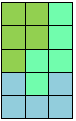
\includegraphics[width=0.9\textwidth]{salida5.png}
\end{center}
\end{figure}



\clearpage

\section{Referencias}


$http://www.minizinc.org/downloads/doc-latest/minizinc-tute.pdf$
$http://ldc.usb.ve/~bonet/courses/ci5437/projects/spring-2015/p3.pdf$

\end{document}
